% Options for packages loaded elsewhere
\PassOptionsToPackage{unicode}{hyperref}
\PassOptionsToPackage{hyphens}{url}
%
\documentclass[
]{article}
\usepackage{amsmath,amssymb}
\usepackage{iftex}
\ifPDFTeX
  \usepackage[T1]{fontenc}
  \usepackage[utf8]{inputenc}
  \usepackage{textcomp} % provide euro and other symbols
\else % if luatex or xetex
  \usepackage{unicode-math} % this also loads fontspec
  \defaultfontfeatures{Scale=MatchLowercase}
  \defaultfontfeatures[\rmfamily]{Ligatures=TeX,Scale=1}
\fi
\usepackage{lmodern}
\ifPDFTeX\else
  % xetex/luatex font selection
\fi
% Use upquote if available, for straight quotes in verbatim environments
\IfFileExists{upquote.sty}{\usepackage{upquote}}{}
\IfFileExists{microtype.sty}{% use microtype if available
  \usepackage[]{microtype}
  \UseMicrotypeSet[protrusion]{basicmath} % disable protrusion for tt fonts
}{}
\makeatletter
\@ifundefined{KOMAClassName}{% if non-KOMA class
  \IfFileExists{parskip.sty}{%
    \usepackage{parskip}
  }{% else
    \setlength{\parindent}{0pt}
    \setlength{\parskip}{6pt plus 2pt minus 1pt}}
}{% if KOMA class
  \KOMAoptions{parskip=half}}
\makeatother
\usepackage{xcolor}
\usepackage[margin=1in]{geometry}
\usepackage{graphicx}
\makeatletter
\def\maxwidth{\ifdim\Gin@nat@width>\linewidth\linewidth\else\Gin@nat@width\fi}
\def\maxheight{\ifdim\Gin@nat@height>\textheight\textheight\else\Gin@nat@height\fi}
\makeatother
% Scale images if necessary, so that they will not overflow the page
% margins by default, and it is still possible to overwrite the defaults
% using explicit options in \includegraphics[width, height, ...]{}
\setkeys{Gin}{width=\maxwidth,height=\maxheight,keepaspectratio}
% Set default figure placement to htbp
\makeatletter
\def\fps@figure{htbp}
\makeatother
\setlength{\emergencystretch}{3em} % prevent overfull lines
\providecommand{\tightlist}{%
  \setlength{\itemsep}{0pt}\setlength{\parskip}{0pt}}
\setcounter{secnumdepth}{-\maxdimen} % remove section numbering
\usepackage{titlesec}
\titleformat*{\section}{\normalfont\Large\bfseries\flushleft}
\titleformat*{\subsection}{\normalfont\large\bfseries\flushleft}
\titleformat*{\subsubsection}{\normalfont\normalsize\bfseries\flushleft}
\usepackage{amsmath}
\newcommand*{\defeq}{\mathrel{\vcenter{\baselineskip0.5ex \lineskiplimit0pt \hbox{\scriptsize.}\hbox{\scriptsize.}}}=}
\newcommand*{\eqdef}{=\mathrel{\vcenter{\baselineskip0.5ex \lineskiplimit0pt \hbox{\scriptsize.}\hbox{\scriptsize.}}}}
\ifLuaTeX
  \usepackage{selnolig}  % disable illegal ligatures
\fi
\usepackage{bookmark}
\IfFileExists{xurl.sty}{\usepackage{xurl}}{} % add URL line breaks if available
\urlstyle{same}
\hypersetup{
  pdftitle={Statistical Learning (5454) - Assignment 3},
  pdfauthor={Matthias Hochholzer, Lukas Pirnbacher, Anne Valder},
  hidelinks,
  pdfcreator={LaTeX via pandoc}}

\title{Statistical Learning (5454) - Assignment 3}
\author{Matthias Hochholzer, Lukas Pirnbacher, Anne Valder}
\date{Due: 2024-05-20}

\begin{document}
\maketitle

\section{Exercise 1}\label{exercise-1}

We load the data set \textit{Carseats} from package \textit{ISLR2}. It
is a simulated data set containing sales of child car seats at 400
different stores. We then select 200 samples (50:50 split) as training
data and use the remaining ones as test data.

We fit a regression tree to the training set. The stopping criterion is
set to \(cp = 10^{-4}\)

\begin{verbatim}
## 
## Regression tree:
## rpart(formula = Sales ~ ., data = train, method = "anova", parms = list(split = "gini"), 
##     control = list(cp = 1e-04))
## 
## Variables actually used in tree construction:
## [1] Advertising Age         CompPrice   Education  
## [5] Population  Price       ShelveLoc  
## 
## Root node error: 1439/200 = 7.2
## 
## n= 200 
## 
##        CP nsplit rel error xerror  xstd
## 1  0.1959      0      1.00   1.01 0.096
## 2  0.1160      1      0.80   0.82 0.077
## 3  0.0674      2      0.69   0.75 0.072
## 4  0.0559      3      0.62   0.75 0.077
## 5  0.0439      4      0.56   0.78 0.078
## 6  0.0323      5      0.52   0.72 0.073
## 7  0.0308      6      0.49   0.69 0.070
## 8  0.0276      7      0.46   0.68 0.069
## 9  0.0230      8      0.43   0.69 0.070
## 10 0.0225      9      0.41   0.67 0.073
## 11 0.0155     10      0.38   0.68 0.076
## 12 0.0147     11      0.37   0.71 0.077
## 13 0.0135     12      0.35   0.69 0.076
## 14 0.0118     13      0.34   0.68 0.075
## 15 0.0070     14      0.33   0.68 0.075
## 16 0.0001     15      0.32   0.68 0.076
\end{verbatim}

The complexity parameter table and the plot of the tree is seen below.

\begin{center}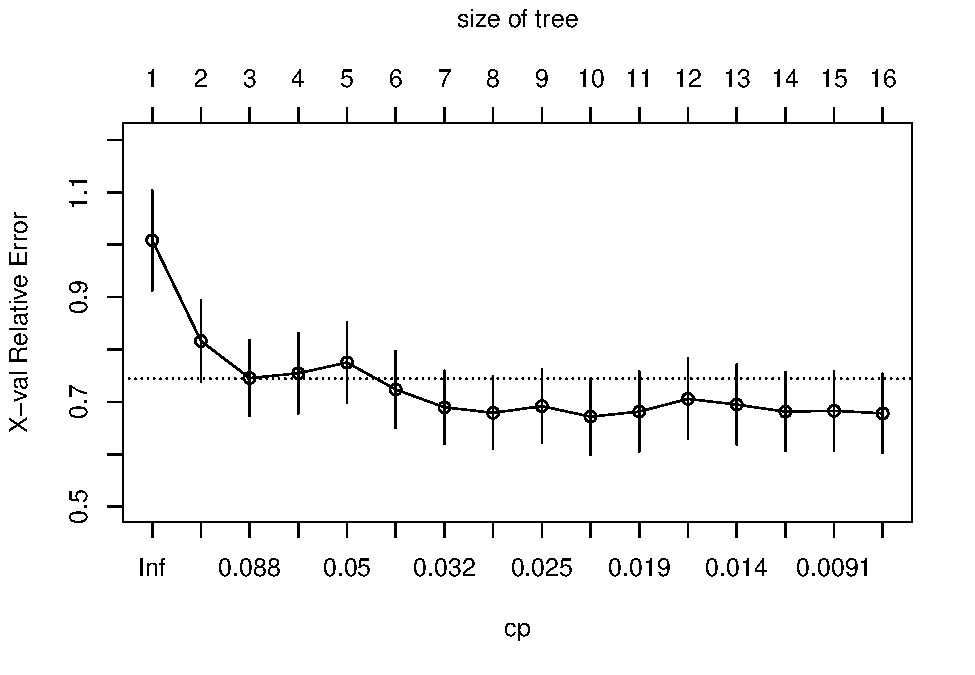
\includegraphics{A3_files/figure-latex/unnamed-chunk-5-1} \end{center}

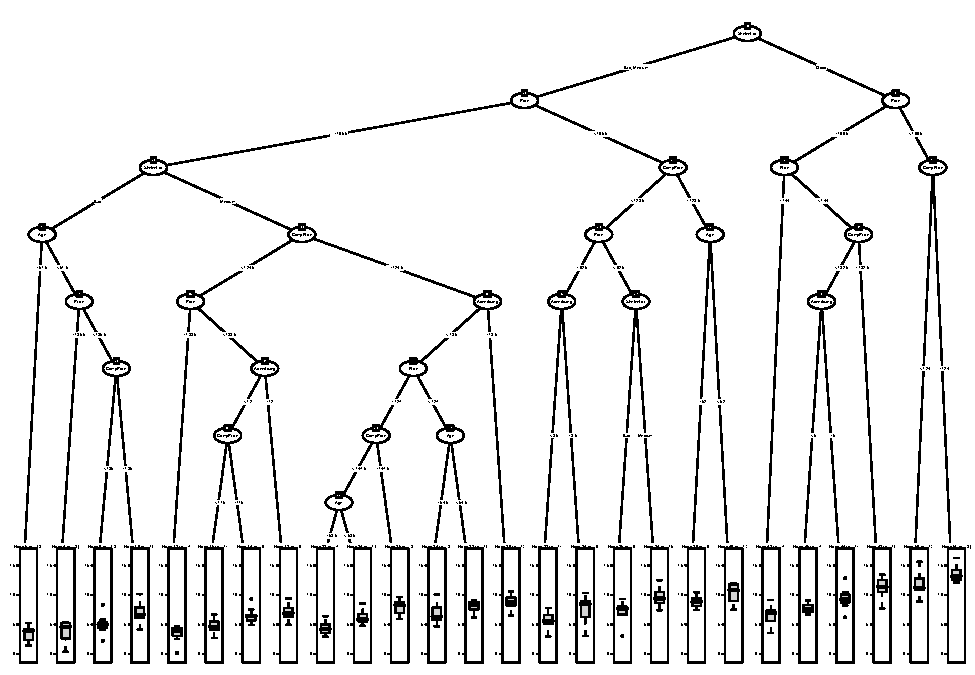
\includegraphics{A3_files/figure-latex/unnamed-chunk-6-1.pdf}

The tree has 16 terminal nods (15 splits). With the loose stopping
criterion we are facing the risk of overiftting. In order to solve this
problem we prune the tree later on. As he \textit{xerrror} doesn't
increase for high \text{cp}, I would already guess that overfitting
isn't a big problem. Since the tree is rather long we do further
interpretations with the pruned tree.

For now, we calculate the test MSE, which is

\begin{verbatim}
## [1] 4.21
\end{verbatim}

Let's use cross-validation in order to determine the optimal level of
tree complexity. To do this, we use the first entry where the
\textit{xerror} is smaller than the minimum error plus one standard
deviation as complexity parameter.
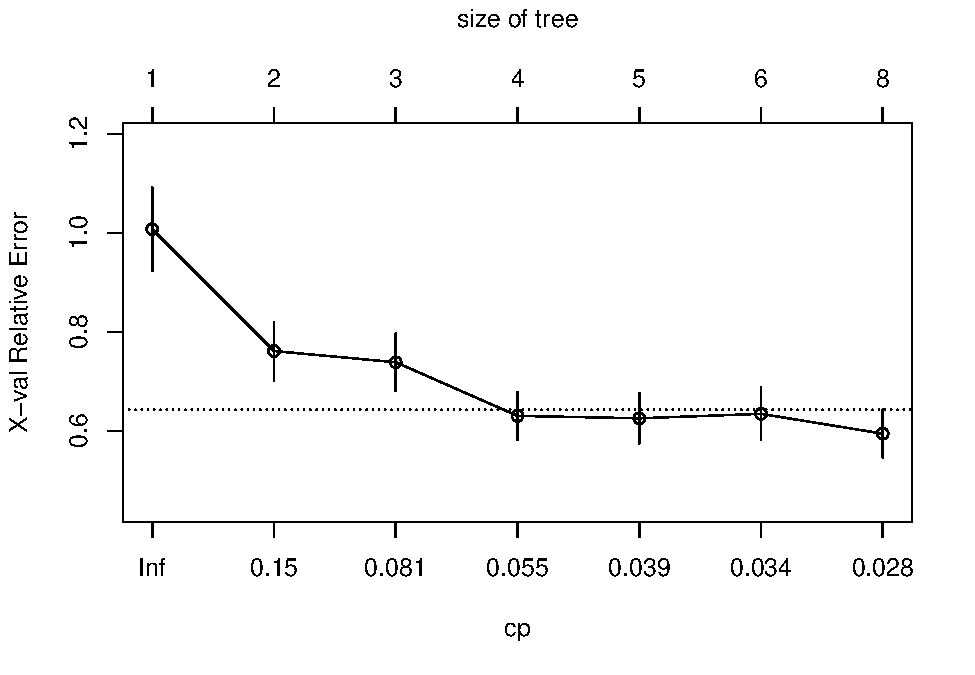
\includegraphics{A3_files/figure-latex/unnamed-chunk-8-1.pdf}
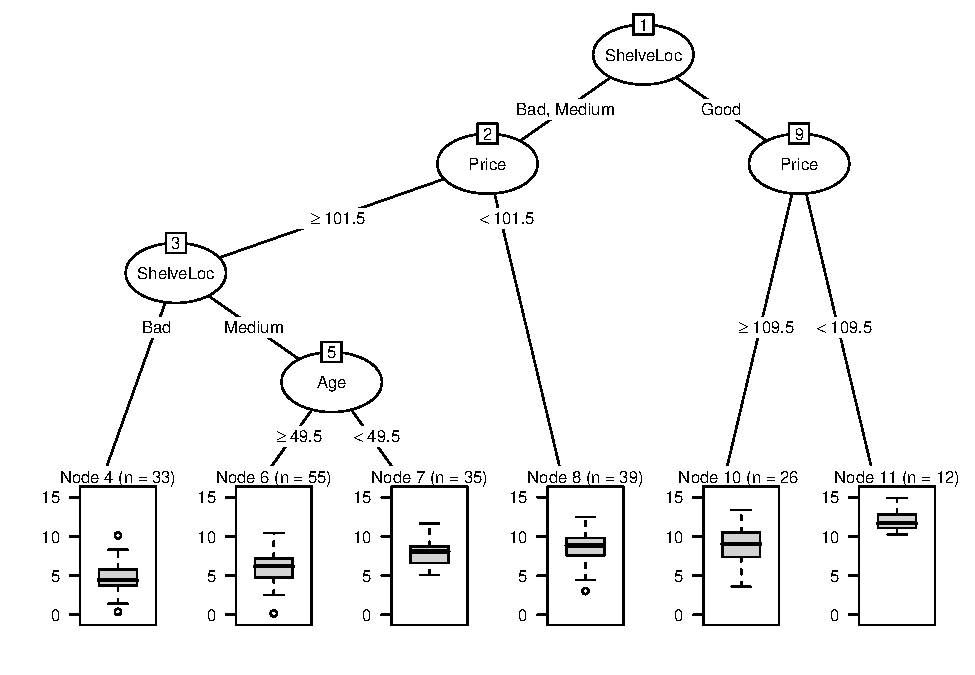
\includegraphics{A3_files/figure-latex/unnamed-chunk-8-2.pdf}

The pruned tree has 6 terminal nods (5 splits). The fist split is done
according to the quality of the shelving location for the car seats. It
splits into \textit{Bad \& Medium} and \textit{Good}. The second split
is the car seat price after a \textit{Bad \& Medium} shelving location.
In the third it's again split by the shelving location. This time
between \textit{Bad} and \textit{Medium}. The next is after a Medium
shelving location according to the average age of the local population.
And lastly by Price after a \textit{Good} shelving location. Looking at
the boxplots, it seems that even the last split was still important.

The test MSE with pruning is

\begin{verbatim}
## [1] 4.669
\end{verbatim}

The test MSE with pruning is higher than without. Therefore pruning the
tree doesn't improve the test MSE. Hence, overfitting was acutally not
too much of a problem.

\section{Exercise 2}\label{exercise-2}

We draw 100 observations from four independent variables \(X_1\),
\ldots{} ,\(X_4\) where

\begin{itemize}
  \item $X_1$ follows a uniform distribution,
  \item $X_2$ follows a standard normal distribution,
  \item $X_3$ follows a Bernoulli distribution with success probability $\pi$ = 0.5,
  \item $X_4$ follows a Bernoulli distribution with success probability $\pi$ = 0.1.
\end{itemize}

We repeat 1000 times the following:

\begin{itemize}
  \item Draw a dependent variable y from a standard normal distribution which is independent of the four independent variables.
  \item Fit a tree stump, i.e., a tree which contains only one split.
  \item Determine which variable was used for splitting.
\end{itemize}

Below is the table of relative frequencies, how often each of the
variables was selected for splitting. We also provide a barplot.

\begin{verbatim}
## 
##    X1    X2    X3    X4 
## 0.460 0.471 0.037 0.032
\end{verbatim}

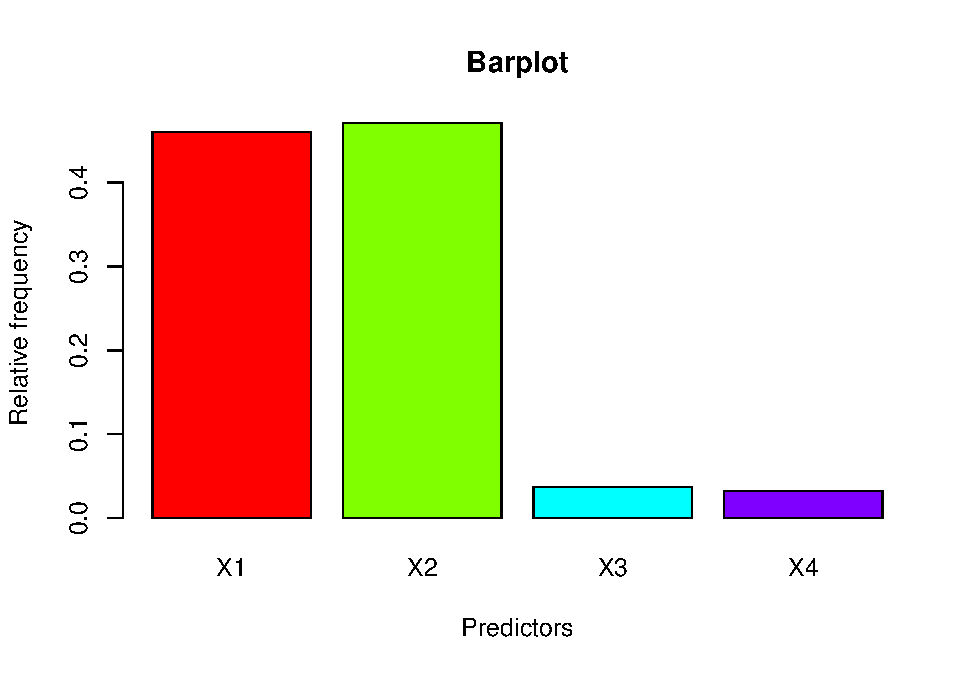
\includegraphics{A3_files/figure-latex/unnamed-chunk-11-1.pdf}

The probability of including a particular independent variable is not
the same. \(X_2\) has the highest probability, closely followed by
\(X_1\). The inclusion probabilities for \(X_3\) and \(X_4\) are much
lower. The different probabilities are a result of the distributions of
the independent variables. It is no great surprise that the highest
inclusion probability occurs for \(X_2\) with its standard normal
distribution when the dependent variable is also standard normally
distributed. The uniform distribution also covers it quite well. The
Bernoulli distribution bears little resemblance to the standard normal
distribution. Therefore, the low inclusion probabilities.

\section{Exercise 3}\label{exercise-3}

Let's assume the following data generating process
\[ Y = X + \epsilon, \] with \(X \sim N(0,1)\) and
\(\epsilon \sim N(0,1)\) independent. In addition 20 covariates
\(Z_1, ... ,Z_{20}\) are given with
\[Z_i \sim \sqrt{0.9}X + \epsilon Z_i ,\] where
\(\epsilon Z_i \sim N(0, 0.1).\)

We draw a training data with 30 observations and a test data with 10,000
observations from the data generating process including the additional
covariates \textbf{Z}.

We then sample 100 bootstrap samples of size 30 from the training data
by drawing with replacement.

To each bootstrap sample we fit:

\begin{enumerate}
\item a regression tree,
\item the null model with predicted value equal to the observed empirical mean of Y ,
\item a linear model including linear effects for X and all Z variables and
\item a linear model potentially including linear effects for X and all Z variables, but using model selection
with the AIC to select a suitable model starting from the null model.
\end{enumerate}

We determine the predicted values on the test data for the bagged model
estimator by calculating the average predictions over the 100 trees
fitted to the bootstrap samples, the 100 null models, the 100 linear
models including all linear effects and the 100 linear models based on
model selection.

Last, we determine the mean squared error (MSE) of the four bagged model
estimators on the test sample of size 10,000.

\begin{verbatim}
##   Model     MSE
## 1  Tree   2.098
## 2  Null   2.114
## 3    LM 377.018
## 4   AIC   2.680
\end{verbatim}

The lowest MSE is achieved by the regression tree, flowed by the null
model and the model selected by AIC. The highest MSE results for the
linear model including X and all Z.

\section{Exercise 4}\label{exercise-4}

We load the dataset icu in package \textbf{aplore3} which contains
information on patients who were admitted to an adult intensive care
unit (ICU). We develop a predictive model for the probability of
survival to hospital discharge of these patients. To fit a predictive
model to the data we use random forests.

We select a suitable number of bootstrap iterations.

Assess the influence of varying the hyperparameter m on the out-of-bag
error obtained and select a suitable value.

Inspect the variable importance measures. Compare the mean decrease Gini
and the mean decrease accuracy measures and assess if the observed
differences in relative importance assigned might be related to the
predictor variable being numeric or not.

\section{Exercise 5}\label{exercise-5}

Assume that there are four predictor variables which have the following
distributions:

\begin{align}
X_1 \sim N(0, 1),&& &X_2 \sim U(0, 1), \\
X_3 \sim M(1, (0.5, 0.5)),&& &X_4 \sim M(1, (0.2, 0.2, 0.2, 0.2, 0.2)).
\end{align}

This means we have two continuous variables which follow either a
standard normal or a standard uniform distribution (\(U(0, 1)\) and two
categorical variables with balanced categories with either 2 or 5
categories, i.e., \(M(N, \pi)\) is the multinomial distribution for N
trials and success probability vector \(\pi\). The dependent variable y
is assumed to be a binary categorical variable with equal-sized
classes.The sample size is set to N = 200.

We generate 100 datasets for each setting and fit a random forest to
each dataset and determine the mean decrease Gini and mean decrease
accuracy values for each of the predictor variables.

Let's suitably visualize the results and interpret them.

\end{document}
